\documentclass[11pt,a4paper]{llncs}
\usepackage{fullpage}


\usepackage{geometry}
\geometry{letterpaper}
\usepackage{graphicx}
\usepackage{amssymb}
\usepackage{epstopdf}
\usepackage{authblk}
\usepackage{wrapfig}
\usepackage{subfig}
\usepackage{hyperref}
\usepackage{amsmath}
\usepackage{appendix}
\usepackage{enumerate}
\usepackage{delarray}
\usepackage{stmaryrd}
\usepackage{tikz}
\usetikzlibrary{fadings,decorations,decorations.pathreplacing}
\DeclareGraphicsRule{.tif}{png}{.png}{`convert #1 `dirname #1`/`basename #1 .tif`.png}
\newcommand{\N}{\mathbb{N}}

\title{Avalanche Structure in the Kadanoff Sand Pile Model
\thanks{Partially supported by  IXXI (Complex System Institute, Lyon) and ANR project  Subtile. }}

\author{Kevin Perrot \and Eric R\'emila}
\institute{Universit\'e  de Lyon\\
  Laboratoire de l'Informatique du Parall\'elisme, \\
  (umr 5668 CNRS - ENS Lyon - Universit\'e  Lyon 1),\\
46 all\'ee d'Italie 69364 Lyon Cedex 7 - France,\\
\email{\{kevin.perrot,eric.remila\}@ens-lyon.fr }}

\begin{document}

\maketitle

\begin{abstract}
  Sand pile models are dynamical systems emphasizing the phenomenon of {\em Self Organized Criticality} (SOC). From  stacked grains, iterating evolution rules leads to some critical configuration where a small disturbance has deep consequences on the system, involving numerous steps of grain fall. Physicists L. Kadanoff {\em et al} inspire KSPM, a model presenting a sharp SOC behavior, extending the well known {\em Sand Pile Model}. In KSPM with parameter  we start from a pile of  stacked grains and apply the rule:  grains can fall from column  onto the  adjacent columns to the right if the difference of height between columns  and  is greater or equal to . We propose an iterative study of KSPM evolution where one single grain addition is repeated on a heap of sand. The sequence of grain falls following a single grain addition is called an avalanche. From a certain column precisely studied for , we provide a plain process describing avalanches.\\
  
\textbf{Keywords:} Discrete dynamical system, self-organized criticality, sand pile model.

\end{abstract}

\section{Introduction}

Sand pile models were introduced in \cite{bak88} as systems presenting a critical self-organized behavior, a property of dynamical systems having critical points as attractors. In the scope of sand piles, starting from an initial configuration of  stacked grains the local evolution of particles is described by one or more iteration rules. Successive applications of such rules alter the configuration until it reaches an attractor, namely a stable state from which no rule can be applied. SOC property means those attractors are critical in the sense that a small perturbation | adding some more grains | involves an arbitrary deep reorganization of the system. Sand pile models were well studied in recent years (\cite{goles93},\cite{durandlose98},\cite{formenti07},\cite{phan08}).


\subsection{Kadanoff sand pile model}

  In \cite{kadanoff89}, Kadanoff proposed a generalization of classical models closer to physical behavior of sand piles in which more than one grain can fall from a column during one iteration. Informally, Kadanoff sand pile model with parameter  and  grains is a discrete dynamical system, which initial configuration is composed of  stacks grains, moving in discrete space and time according to a transition rule : if the height difference between column  and  is greater or equal to , then  grains can fall from column  to the  adjacent columns on the right (see figure \ref{fig:rule}).

\begin{figure}[!h]
  \begin{center}
    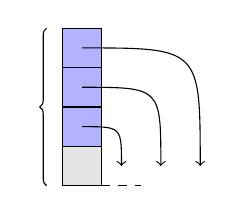
\begin{tikzpicture}
  \foreach \y in {1,...,3}
    \filldraw[fill=blue!30] (0,.5*\y) rectangle ++ (.5,.5);
  \filldraw[fill=black!10] (0,0) rectangle ++ (.5,.5);
  \draw[dashed] (.5,0) -- ++ (.5,0);
  \draw[decorate, decoration=brace] (-.2,0) -- node [left] {} ++ (0,2);
  \draw[->] (.25,.75) .. controls (.75,.75) .. (.75,.25);
  \draw[->] (.25,1.25) .. controls (1.25,1.25) .. (1.25,.25);
  \draw[->] (.25,1.75) .. controls (1.75,1.75) .. (1.75,.25);
\end{tikzpicture}   \end{center}
  \caption{KSPM() transition rule.}
  \label{fig:rule}
\end{figure}


Sand pile models are specializations of {\em Chip Firing Games} (CFG). A CFG is played on a graph in which each vertex  has a load  and a threshold deg^+(v)v, and the transition rule is: if  then  gives one unit to each of its neighbors (we say  is fired). As a consequence, we inherit all  properties of CFGs. 

Kadanoff sand pile is referred to a {\em linear chip firing game} in \cite{goles02}. The authors show that the set of reachable configurations endowed with the order induced by the successor relation has a lattice structure, in particular it has a unique {\em fixed point}. Since the model is non-deterministic, they also prove \emph{strong convergence} {\em i.e.} the number of iterations to reach the fixed point is the same whatever the evolution strategy is. The morphism from KSPM(3) to CFG is depicted on figure \ref{fig:lcfg}.

  \begin{figure}[!h]
  \begin{center}
    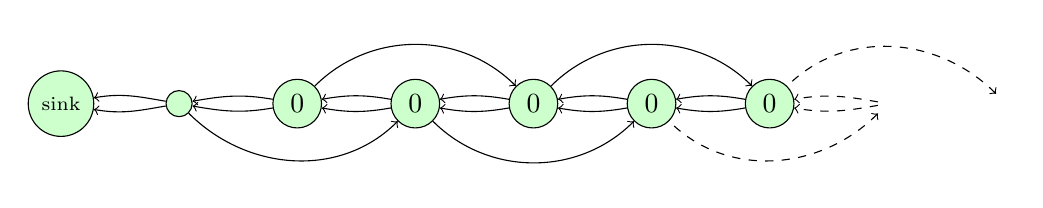
\begin{tikzpicture}
  \node[circle, draw, fill=green!20] (n0) at (0,0) {};
  \node[circle, draw, fill=green!20] (n-1) at (-1.5,0) {\scriptsize sink}
    edge [<-,out=10,in=170] (n0)
    edge [<-,out=-10,in=-170] (n0);
  \node[circle, draw, fill=green!20] (n1) at (1.5,0) {0}
    edge [->,out=170,in=10] (n0)
    edge [->,out=-170,in=-10] (n0);
  \node[circle, draw, fill=green!20] (n2) at (3,0) {0}
    edge [->,out=170,in=10] (n1)
    edge [->,out=-170,in=-10] (n1)
    edge [<-,out=-135,in=-45] (n0);
  \node[circle, draw, fill=green!20] (n3) at (4.5,0) {0}
    edge [->,out=170,in=10] (n2)
    edge [->,out=-170,in=-10] (n2)
    edge [<-,out=135,in=45] (n1);
  \node[circle, draw, fill=green!20] (n4) at (6,0) {0}
    edge [->,out=170,in=10] (n3)
    edge [->,out=-170,in=-10] (n3)
    edge [<-,out=-135,in=-45] (n2);
  \node[circle, draw, fill=green!20] (n5) at (7.5,0) {0}
    edge [->,out=170,in=10] (n4)
    edge [->,out=-170,in=-10] (n4)
    edge [<-,out=135,in=45] (n3);
  \node (n6) at (9,0) {}
    edge [->,dashed,out=170,in=10] (n5)
    edge [->,dashed,out=-170,in=-10] (n5)
    edge [<-,dashed,out=-135,in=-45] (n4);
  \node (n7) at (10.5,0) {}
    edge [<-,dashed,out=135,in=45] (n5);
\end{tikzpicture}   \end{center}
  \vspace{-.5cm}
  \caption{The initial configuration  of KSPM(3) is presented as a CFG where each vertex corresponds to a column (except the sink) seen as a difference of height.}
  \label{fig:lcfg}
\end{figure}

  More formally, sand pile models we consider are defined on the space of ultimately null decreasing integer sequences. Each integer represents a column of stacked sand grains and transition rules describe how grains can move from columns. Let  denote a {\em configuration} of the model, where each integer  is the number of grains on column . Configurations can also be given as height difference , where for all . We will use this latter representation throughout the paper, within the space of ultimately null non-negative integer sequences.


\begin{definition}
The   Kadanoff sand pile model with parameter , KSPM(), is defined by:
  \begin{itemize}
    \item A set of \emph{configurations}, consisting in ultimately null non-negative integer sequences.
    \item A set of \emph{transition rules} : we have a transition from a configuration  to a configuration  on column , and we note    if  
    \begin{itemize}
\item  (for )
\item , 
\item 
\item  for . 
\end{itemize}

  \end{itemize}
\end{definition}

Remark that according to the definition of the transition rules, a condition for  to be a configuration is that .

\subsection{Strategies and avalanches}


A basic property of the KSPM model is the \emph{diamond property}. If there exists two distinct integers  and  such that 
 and , then there exists a configuration  such that   and . 
We  note  when there exists an integer  such that . 
We define the transitive closure  of , and say that  is {\em reachable} from  when  .

A {\em strategy} is a sequence . We say that  is {\em reached} from  via  when  and we note . 
We also say,  for each integer  such that , that the column  \emph{is fired} at \emph{time}  in . (informally,  the index of the sequence is interpreted as time). 

 For any strategy  and any nonnegative integer , we state .  Let   ,  be  two strategies such that  and .  We have the equivalence:  .
 A strategy  such that  is called {\em leftmost} if it is the minimal strategy from  to  according to lexicographic order. A leftmost strategy is such that at each iteration, the leftmost possible transition is performed. 

We say that a configuration  is \emph{stable}, or a \emph{fixed point} if no transition is possible from . 
As a  consequence of the diamond property, one can easily check that, for each configuration , there exists a unique stable configuration, denoted by , such that  . Moreover,  for any  
configuration  such that , we have  (see \cite{goles02} for details). 

In this paper, we are interested in the iterative process defined below. Starting with no grain, we successively add a single  grain on  column 0, and make all the possible firings until  a fixed point is reached. We denote by  the configuration obtained with this process using  grains (from the structure of KSPM described above, one easily checks that ).  


Let  be a configuration,  is the configuration obtained by adding one grain on column . In other words, if , then . 

Formally the process is defined by  and the recurrence formula: 



The {\em  avalanche}  is  the leftmost strategy from  to . 
The goal of the present paper is the description of avalanches. Informally, we want to describe what happens when a new grain is added in a previously stabilized sand pile.  


For , i.e.  the classical SPM, this description is easy: the added grain moves rightwards until it arrives in a plateau. But, for ,  the situation is not so simple. We now state our results. 

 \begin{itemize}
\item In the general case, we prove (Section \ref{section:avalanche}) the following properties:  
 \begin{itemize}
\item Each column is fired at most once, 
\item For any avalanche, as soon as an interval   of successive fired columns exists, the execution of the avalanche on the right part of this interval can be turned into a pseudo local  and elementary process. 

\end{itemize}
Informally, that means that the knowledge of such an interval guarantees a regular behavior  of the avalanche on its right part. 

\item  In the case when ,  we prove (Section \ref{section:bounding}) the property below: 
\begin{itemize}
\item For each avalanche , there  exists an integer   in  such that either no column is fired on the right of ,  or  columns  and  both are fired (and therefore, the property of the second item above applies). 
\end{itemize}
Informally, that means that we have the emergence of  a regular behavior, after a short transitional and complex phase. 
\end{itemize}

These results give a better understanding of avalanches for sufficiently large columns. We hope that in future work, they will help us in the  approach of the structures of fixed points . 

\subsection{The context}

 The problem of describing and proving regularity properties, experimentally checked,  for   models issued from  basic dynamics is really a present challenge for physicists, mathematicians, and computer scientists. There exists
a lot of conjectures, issued from simulations, on  discrete dynamical systems with simple local rules (sandpile model \cite{dartois} or chip firing games, but also  rotor router  \cite{levine},  the famous Langton ant\cite{gajardo}\cite{propp}...)  but very few results have actually been proved. As regards KSPM(), the {\em prediction problem} (namely, the problem of computing the fixed point  knowing ) has been proven in \cite{moore99} to be in \textbf{NC} for the one dimensional case (the model of our purpose), which means that the time needed to compute an avalanche is in  where  is the number of grains, and \textbf{P}-complete when the dimension is .  A recent study (\cite{goles10}) showed that in the two dimensional case the avalanche problem (given a configuration  and a column  on which we add one grain, does it have an influence an index ?) is \textbf{P}-complete, which points out a inherently sequential behavior.

This study will provide tools to understand sand pile evolution. We hope that those tools form a basis to obtain  some good descriptions of fixed points , but are also deeply related with other subjects around sand piles such as unit elements of abelian group structures presented 
in \cite{creutz96} and \cite{dhar90}.

\section{Avalanche process in the general case}\label{section:avalanche}

This section begins with a first glance at avalanches, allowing notation simplifications. Then avalanches are studied in details, leading to a simplified description of its behavior.

\begin{proposition}\label{lemma:01}
  For each strategy   such that   and  each  , we have  . 
\end{proposition}

\begin{proof}
  Let  be a strategy such that  . We have to  prove  that, for  
  , we have  (obviously,  for all ). To do it,  we prove by induction  that for
, we have .\\ 
  For initialization this is obviously true for . 
   Now assume that the condition is satisfied for an integer  such , and let  be a column such that there exists an integer  such that . Let   be the  configuration such that .\\
  Notice that the transitions which can possibly change the value of the current configuration at  could be:  (which decreases the value by  units),  (which increases the value by  units) or   (which increases the value by  unit).\\
  Thus we have  since by definition,  between    and , exactly one transition has occurred in   , at most one transition has occurred in , and at most one transition has occurred in . For , we get . On the other hand, since  is a fixed point, we have:   ,  which guarantees that . For , there is no possible transition in , thus we get , which is  . Thus     which also gives: .\\
  This ensures that the result is true for ,  and,  by induction,  for . 
\end{proof}

When talking about an avalanche , lemma \ref{lemma:01} allows us to write  instead of  without lose of information. We denote by    the  subsequence of  from   to  included.

We will now study avalanches in details. For , i.e.  the classical SPM, avalanches are quite simple, the added grain moves rightwards until it finds a stable position. For , the situation is more complex, and needs a precise study, given by the following lemma.  


\begin{lemma}\label{lemma:localdensity}
Let  be the  avalanche. Let .
\begin{itemize}
\item Assume that .  Then   is the largest column number  such that  and . Moreover,  we have: .
\item Assume that . We have:  .
\end{itemize}

\end{lemma}

\begin{proof}
We first order fired columns by causality. Precisely, a column  has  two potential predecessors, which are
 and   . State . These columns are really predecessors of  if they are elements of , i.e if they are fired before . By this way, using the transitive closure,  we define a partial order relation (denoted by ),  on fired columns for .

Now,  consider the set  of ancestors of  (i.e.  the set of columns  such that )  and,    the set  of which have   as common ancestor (i.e. columns  such that ).
We necessarily have  .   Otherwise, we have  , and this  allows  another strategy , constructed from  postponing the transitions at   and elements of  after the transition on  . This contradicts the fact that  is leftmost.

Let   be a finite sequence such that ,  and,  for each  with ,  is a predecessor of . Such a sequence exists since . One easily proves by induction that : 
this is true for . Assume it is true until the integer . We have either  or  . But from the induction hypothesis,  is an ancestor of  or has not yet been fired, thus .  This gives that     is the largest column number  such that  and . 

Now if we assume, by contradiction, that  , then   is not a predecessor of , which yields that  has no predecessor, which is a contradiction. This gives the  inequality   of the first item. 
The second item  is obvious, since  ha a unique predecessor which is . 
\end{proof}

Lemma \ref{lemma:localdensity} induces a partition of fired columns between those which make a progress ({\em i.e.} increases the greatest fired column) and those which do not. This distinction is important in further development, so let us give progress firings a name. Let  be an avalanche, a column  is called a {\em peak} if and only if .

\begin{remark}\label{remark:order}
  Two peaks  can be compared using chronological () or spatial () orders. Nevertheless, by definition of peaks we obviously have .
\end{remark}

\begin{lemma}\label{lemma:D-1}
  Let  be the  avalanche. Assume that  there exists a column  ,  such that for each column   with , , and a column  such that  and . Let   be  the lowest peak such that  .
  
There exists a time   such that:

 \begin{tabular}[t]\{{l}. 
 for all  with , \\
  for all  with , 
   \end{tabular}
   
  Moreover  is the lowest integer such that   and . 
\end{lemma}

\begin{proof}

 Let  be the time when , i.e. the   first  time such that ,  and let  be the largest integer such that,  for , we have .  Let us state . We have . \\
Let  denote the configuration obtained from  via . Let   , with ,  such that . We claim that we have :  . To prove it, we prove by induction that for any ,  . Assume that this is satisfied for a fixed . This means that all the transitions of   are done on columns larger than .  Thus,  and no transition is possible  on  for  since   is leftmost (the only potential column to be fired is , but by assumption, either this column has been previously fired,  or it cannot be fired by definition of , according to lemma \ref{lemma:localdensity}) . \\
By contraposition,  it follows that for each column   with ,  we have .  A   simple (reverse sense) induction shows that,   for    we have , since  by hypothesis , and  both are in .  Thus, by contraposition of the claim above,  for ,   we have . 
This gives  the the fact that for all  with , \\
The fact that for all  with ,  is trivial,  by definition of  and .\\
 We have  and . assume that there exists  satisfying the same properties. Notice that 
 for    we have . Thus the time  such that   is such that . 
  That means that   should have been fired before ,  a contradiction.
\end{proof}

Lemma \ref{lemma:D-1} describes in a very simple way the behavior of avalanches. Thank to it, the study of an avalanche can be turned into a pseudo linear execution, in which transitions are organized in a clear fashion:




\begin{theorem}\label{corollary:peak}
  Let  be the  avalanche and  be its sequence of peaks. Assume that  there exists a column ,  such that for each column   with , . 
  Then for any column  such that , 
  
  
  Furthermore, Let , with , be a peak. Then
  

 \end{theorem}

 A graphical representation of this statement is given on figure \ref{fig:peak}.

\begin{proof}
  The first part  is a straight induction on lemma \ref{lemma:D-1}.\\
  The second part follows an induction summed up in the following fact: any column  such that  must wait for its right neighbor  to be fired, and it should be fired when both  and  has been fired (besides,  has already been fired). Since any of such  is fired to reach a fixed point, .
\end{proof}

\begin{figure}
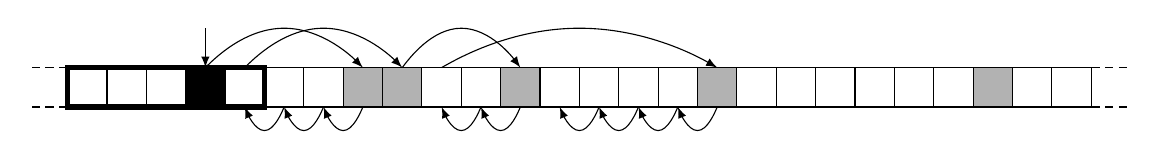
\begin{tikzpicture}
  \filldraw[fill=black] (3*.5,0) rectangle ++ (.5,.5);
  \foreach \x in {7,8,11,16,23}
    \filldraw[fill=black!30] (\x*.5,0) rectangle ++ (.5,.5);
  \foreach \x in {0,...,25}
    \draw (\x*.5,0) rectangle ++ (.5,.5);
  \draw[densely dashed] (13,0) -- ++ (.5,0);
  \draw[densely dashed] (13,.5) -- ++ (.5,0);
  \draw[densely dashed] (0,0) -- ++ (-.5,0);
  \draw[densely dashed] (0,.5) -- ++ (-.5,0);
  \draw[line width=2pt] (0,0) -- ++ (2.5,0) -- ++ (0,.5) -- ++ (-2.5,0) -- cycle;
  \node at (.25,-.25) {};
  \draw[-latex] (3*.5+.25,1) -- ++ (0,-.5);
  \draw[-latex] (3*.5+.25,.5) parabola[bend pos=0.5] bend +(0,.5) +(4*.5,0);
  \draw[-latex] (4*.5+.25,.5) parabola[bend pos=0.5] bend +(0,.5) +(4*.5,0);
  \draw[-latex] (8*.5+.25,.5) parabola[bend pos=0.5] bend +(0,.5) +(3*.5,0);
  \draw[-latex] (9*.5+.25,.5) parabola[bend pos=0.5] bend +(0,.5) +(7*.5,0);
  \foreach \x in {5,6,7,10,11,13,14,15,16}
    \draw[-latex] (\x*.5+.25,0) parabola[bend pos=0.5] bend +(0,-.3) +(-.5,0);
\end{tikzpicture}
\caption{Illustration of Theorem \ref{corollary:peak} with . Surrounded columns  to  are supposed to be fired. Black column is the greatest peak strictly lower than . A column is grey if and only if its value is . Following arrows depicts the avalanche.}
\label{fig:peak}
\end{figure}

  In the light of remark \ref{remark:order}, theorem \ref{corollary:peak} easily allows us to compute the right part of  avalanche (from column ), only knowing . The sequence of peaks is computed as follows. The first one is the lowest column  greater or equal to  such that . Then, given a peak , the next one is the lowest   such that   and . If such a  does not exist, then there is no more peak and  is the largest fired column.

  We can distinguish two movements within an avalanche: before a certain column it has an unknown behavior, and from that column to the end the behavior is pseudo local, in the sense that when an index is fired ahead (on the right) then any `hole' is filled before the progress can continue.

An important direct implication of theorem \ref{corollary:peak} is that if there exists a column  such that for the  avalanche , we have for all , , then for all  such that , we have  and therefore . Intuitively, this equality hints some similarity between successive avalanches.

Note that previous results also apply for a grain addition on column 0 of any fixed point configuration of KSPM().

This study constitutes a simplified understanding of the behavior of avalanches, which we hope will be helpful toward the description of fixed points. As motivated above, next subsection studies, for KSPM(3),  the previous result hypothesis  that for an avalanche  there exists a column  such that for all ,  is element of .\\
    
\section{Short transitional phase when }\label{section:bounding}

In this section we prove that in KSPM(3), there exists a column  in  such that lemmas hypothesis is verified for any avalanche , with , such that . In other words, considering the  first avalanches, from a logarithmic column,  we can apply theorem \ref{corollary:peak} and consider avalanches pseudo locally, as described on figure \ref{fig:peak}. Here is the statement:

\begin{proposition}\label{lemma:meta2}
Let  be the  avalanche of KSPM(3). There exists a column  in  such that for any , when  ,  and  both are elements of .
\end{proposition}

\begin{proof}

Let  be a fixed column. If , then, theorem \ref{corollary:peak} states that for all  such that , we have . If , then, from Proposition \ref{lemma:localdensity},  we have .

 Let  be a fixed positive integer. Assume  that  the avalanche  fires  but not . From remarks above, columns  are fired in  while  columns  are not fired. 
 
 
If a column  is fired while  is not, then we necessarily have ,  since the firing in  increases the value in column  from 2 units. 
Moreover, if the  column  is fired while  is not, then we necessarily have , since the   receives at most one grain, by preceding firings. 

On the other hand,  obviously, the assumption on  enforces that   
This yields that  is a prefix  of . 

We have the following fact : \\ 

\textbf{Fact:} 
There exists constant numbers  and , with  such that if a  configuration   has a prefix of the form  then \\
 
 This is obtained by  the  linear algebra analysis below. This gives the result of the proposition.  


 Let  be the  configuration and  be its 
 {\em shot vector} i.e.   the sequence   where  is the number of times the column   has be fired in the  first avalanches. According to the iteration rule we have the relation:
 
 
 i.e.   

We state  . We denote  by  the column vector such that  and 
and     the column vector such that  (with the convention that   is  the row vector   obtained by transposition of the column vector ) . The equality above can be algebraically written in

 

By
iteration we get :



What we want is  and  so  and . With this specification, we get : 



 with .
From this last relation we will deduce a condition on  to get the sequence .\\


Let us first find a new basis to get the matrix  on Jordan canonical form. The characteristic polynomial of  is  and its eigenvalues are  of algebraic multiplicity 1 and 1 of algebraic multiplicity 2. Since  the Jordan canonical form of A is

And the new basis  according to the canonical one  is given by the linear relations:
\begin{center}
 \begin{tabular}{l}
   \\
   \\
   
 \end{tabular}
\end{center}

Let  be  the
 linear mapping consisting in the projection on the line  generated  by   according to the direction the plane   generated by  and . For any vector , we have:  . Notice that, by definition of ,  is element of , and,  therefore  and  also are elements of . This yields that  is null.
 On the other hand, since   is element of ,  and ;  thus  . As a conclusion, we get , which, in particular, allows the following equalities:

\begin{center}
 \begin{tabular}{rl}
    & \\
    & \\
    & 
 \end{tabular}
\end{center}
Let  be the unique vector collinear with  satisfying the equation

i. e.  .  Remember that . We have
\begin{center}
 \begin{tabular}{rl}
    & \\
    & \\
    & 

 \end{tabular}
\end{center}
This gives by induction: 



Now we specify the sequence of vectors ,  assuming that values  are the shot vectors of a configuration  beginning by .
 (For convention we also  state  and , thus we have ,  and  for ).

 An easy computation gives that:  
 

 Let  be defined by . We obtain   the equality :



Obviously , which ensures that  .

Furthermore,  we necessarily have , and, from lemma \ref{lemma:alpha} proved on the bounce, each element of  is a multiple of , where  is a positive constant.
If   is element of   we can conclude that 
If   is not element of  ,  we can conclude that . In any case,  there exists a positive real , not depending on ,   such that  


We conclude that , which gives  to get a sand pile of the form .
\end{proof}

We now give the lemma used in the previous proof. 

\begin{lemma}(constant steps)\label{lemma:alpha}
  There exists a  positive real  such that .
\end{lemma}

\begin{proof}
  The set  of reals  such that there exists an element  in  such that   is obviously a group. So we only have to prove that this group is discrete, {\em i.e.} that there is no sequence  of positive reals such that .\\
 Assume, by contradiction, the existence of such a sequence, and let   be a sequence of vectors such that, for each integer , . \\
 A key-point is that vectors ,  and  have  integer  components, so we can state . 
 The sequence   defined by   
 also is a sequence of integer vectors such that for each integer , . Moreover this sequence is bounded. Thus  takes a finite number of values, which enforces that the sequence  also takes a finite number of values, which is a contradiction. 
\end{proof}

For KSPM(3), after a short transitional of logarithmic length,  hypotheses of theorem \ref{corollary:peak} are verified , and the study of avalanches can be turned into a pseudo linear process. Note that a trivial framing of the maximal non-empty column  of a fixed point with  grains shows that  is in . As a consequence, pseudo local process stands for the asymptotically complete behavior of avalanches.\\



Unfortunately, the approach above does not hold for .  The main reason is that, for  unfired columns induce a very particular and \emph{periodic} prefix () on configurations. From , the structure of such a possible prefix is more complex and we did not yet get a tractable characterization of those prefixes. 

\section{Perspectives}

In this paper we described avalanches as pseudo local processes from a certain column .

We proved this column to be logarithmic in the number of grains  for KSPM(3), leading to an asymptotically complete description of avalanches in that case. Simulations for other parameter  suggests that the same outcome also holds.

The pseudo local process description involves some properties on avalanches, which we hope will be useful toward the study of fixed points shape. For an avalanche , a particularly interesting consequence is that two successive fixed points are equal from  to , which hints that next avalanche reaching this part of the configuration may have a similar behavior. This would lead to a knowledge on the likeness of successive avalanches and therefore a foresee on the shapes of fixed points. Further work may concentrate on this point, where the main purpose is to go ahead iterating evolution rules, and to describe fixed points with a plain formula.

\bibliographystyle{plain}
\bibliography{biblio}

\end{document}
